% https://nl.mathworks.com/help/autoblks/ref/fluxbasedpmcontroller.html
% https://www.researchgate.net/publication/268355311_Nonlinear_State-Observer_Techniques_for_Sensorless_Control_of_Automotive_PMSM's_including_Load-Torque_Estimation_and_Saliency
% https://www.miniquadtestbench.com/brushless-drive-and-esc-basics.html
% https://support.controltechnologycorp.com/customer/elearning/younkin/motorParameters.pdf
% https://www.ti.com/lit/an/sprabq3/sprabq3.pdf?ts=1608197151612
% https://ir.lib.uwo.ca/cgi/viewcontent.cgi?article=4159&context=etd
% https://www.ti.com/lit/an/spraby9/spraby9.pdf?ts=1608924152407&ref_url=https%253A%252F%252Fwww.google.com%252F

% https://nl.mathworks.com/help/physmod/sps/ug/three-phase-pmsm-drive.html?searchHighlight=Three-Phase%20PMSM%20Drive&s_tid=srchtitle

% https://www.youtube.com/watch?v=xFCBQTuMOa0&list=PLl6mqZGq1o09k59iLGNs7AdLuJi9FoVcV&index=6

% https://www.maxongroup.nl/medias/sys_master/root/8841181265950/EN-207.pdf + https://www.maxongroup.nl/maxon/view/category/motor?etcc_cu=onsite&etcc_med_onsite=Product&etcc_cmp_onsite=EC+programma&etcc_plc=Overview-Page-brushless-DC-Motors&etcc_var=%5bnl%5d%23nl%23_d_&target=filter&filterCategory=ec
% https://www.maxongroup.fr/medias/sys_master/root/8837129142302/maxonECmotor-Notes.pdf?attachment=true
% https://www.maxongroup.com/medias/sys_master/8803450814494.pdf?attachment=true

% https://www.maxongroup.nl/medias/sys_master/root/8841185067038/EN-276.pdf (339252) + https://www.maxongroup.nl/maxon/view/category/motor?etcc_cu=onsite&etcc_med_onsite=Product&etcc_cmp_onsite=EC+flat+programma&etcc_plc=Overview-Page-brushless-DC-Motors&etcc_var=%5bnl%5d%23nl%23_d_&target=filter&filterCategory=ecflat 
\documentclass[]{report}
\usepackage[english]{babel}
\usepackage[backend=bibtex]{biblatex}
\usepackage{graphicx}
%\usepackage{subfig}
\usepackage{float}
\usepackage{hyperref} %[hidelinks]
\usepackage{xcolor}
\usepackage{wrapfig}
\usepackage{gensymb}
\usepackage{amsmath}  \setcounter{MaxMatrixCols}{16}
\usepackage{caption}
\usepackage{subcaption}

\hypersetup{
	colorlinks,
	linkcolor={red!50!black},
	citecolor={blue!50!black},
	urlcolor={blue!80!black}
}

\graphicspath{ {../Img/} }
\addbibresource{../BLDC_ESC_Control_Bib.bib}

\title{	\huge Field Oriented Control for BLDC motors \\
		\large Project execution \\ 5LIU0}
\author{Enzo Evers}

\pagestyle{plain}

\begin{document}
\maketitle
\tableofcontents

\newpage

\begin{tabular}{|l|l|}
	\hline
	BLDC & Brushless Direct Current \\
	\hline
	PMSM & Permanent Magnet Synchronous Motor \\
	\hline
	BEMF & Back Electromotive Force \\
	\hline
	FOC & Field Oriented Control \\
	\hline
	SVM & Space Vector Modulation \\
	\hline
	ESC & Electronic Speed Controller \\
	\hline
	FC & Flight Controller \\
	\hline
	DMA & Direct Memory Access \\
	\hline
	FPV & First Person View \\
	\hline
	RC & Radio Controlled \\
	\hline
	RPM & Rotations Per Minute \\
	\hline
	SMO & Sliding Mode Observer \\
	\hline
	UKF & Unscented Kalman Filter \\
	\hline
\end{tabular}

\newpage

\chapter{Introduction}
% A general description of your project and its challenges.

In this project an FOC system will be created for BLDC motors. BLDC motors are used in a lot of this. From factories to house appliances to vehicles. But also in Radio Controlled (RC) vehicles. First Person View (FPV) drones also used BLDC motors. Controlling a BLDC motor with a microcontroller requires an Electronic Speed Controller (ESC). These electronic speed controllers require firmware to translate the incoming control signal to voltages which are applied to the motor. For FPV drones most of the firmware however is closed source. This project aims to design a controller which can be used to drive BLDC motors and help the open source ESC projects such as AM32 \cite{AM32_Git}.

\chapter{Problem specification}
% A detailed and technical description of the problem you’re addressing.

In this project the Field Oriented Control (FOC) algorithm will be used to drive a sensorless Brushless Direct Current (BLDC) motor used in the Radio Controlled (RC) vehicle hobby. FOC is generally not used the RC hobby because it requires more information about the driven motor and requires higher precision in the controller, compared to the six-step commutation method. More information about the six-step commutation method and how these signals in RC vehicles look can be found in the project proposal for this project \cite{Project_Proposal_EnzoEvers_FOC_BLDC}.

\section{Why Field Oriented Control}
FOC is different from six-step commutation in two main ways:
\begin{enumerate}
	\item FOC uses (PWM modulated) sinusoidal voltages on all 3 phases during operation instead of (PWM modulated) block voltages on 2 phases at a time during operation used in six-step commutation.
	\item FOC aims to create a magnetic field in the stator with a constant 90\degree lead with respect to the rotor flux for maximum constant torque. In six-step commutation the magnetic field in the stator goes from 60\degree to 120\degree in each commutation step, resulting in a torque ripple.
\end{enumerate}

\section{Steps in Field Oriented Control}
% https://www.youtube.com/watch?v=UC5XjoHNQisz`
% Clarke
% Park

\autoref{fig:FOC_Coordinate_systems} shows the three different coordinate systems used in FOC.

\begin{figure}[H]
	\centering
	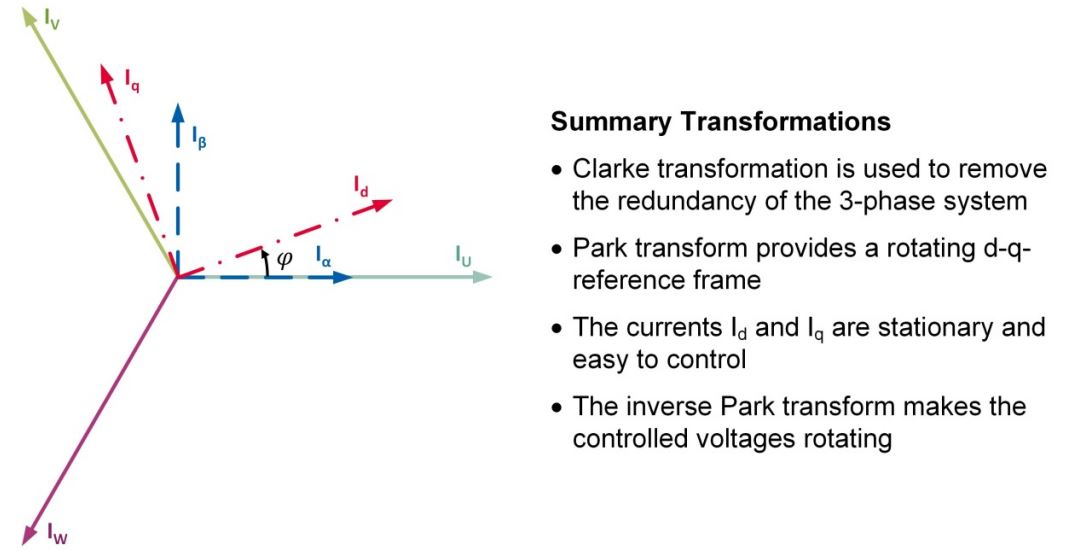
\includegraphics[width=\textwidth]{CoordinateSystems.JPG}
	\caption{The three different coordinate systems used in FOC \cite{Infineon_sensorless_FOC}}
	\label{fig:FOC_Coordinate_systems}
\end{figure}

\subsubsection{Clarke transform}
The three arrows which are 120\degree separated ($I_U$, $I_V$, $I_W$) represent the three motor phases. The current in each phases is represent using a vector. Since this is a 2D plane the vector can also be represent using a 2-axis system. This is the $\alpha\beta$ systems and is obtained using the Clarke transform. The (magnitude invariant) Clarke transform in is shown below (\autoref{eq:ClarkeTransformMatrix}) and uses the phase names shown in \autoref{fig:FOC_Coordinate_systems}. The values in the transformation matrix on the first row (the row for $I_\alpha$) represent the cosine values for $cos(0\degree), cos(120\degree), cos(-120\degree)$ respectively. Indicating how much each phase adds to the $\alpha$ axis. The values on the second row (the row for $I_\beta$) represent the sine values for $sin(0\degree), sin(120\degree), sin(-120\degree)$ respectively.

% https://www.cypress.com/file/222111/download

% Matlab_Simulink_Math_transforms

\begin{equation} \label{eq:ClarkeTransformMatrix}
\begin{bmatrix} I_\alpha \\ I_\beta \end{bmatrix}
= \frac{2}{3} 
\begin{bmatrix}
	1 && -\frac{1}{2} && -\frac{1}{2} \\
	0 && \frac{\sqrt{3}}{2} && -\frac{\sqrt{3}}{2}
\end{bmatrix}
\begin{bmatrix} I_U \\ I_V \\ I_W \end{bmatrix}
\end{equation}

Using Kirchhoff's current law for the three phase currents ($0 = I_U + I_V + I_W$), \autoref{eq:ClarkeTransformMatrix} can be rewritten to \autoref{eq:ClarkeTransformSimplified}. This shows that only two phases have to be measured.

\begin{equation} \label{eq:ClarkeTransformSimplified}
\begin{split}
	I_\alpha &= I_U \\
	I_\beta &= \frac{1}{\sqrt{3}} (I_U + 2I_V)
\end{split}
\end{equation}

\label{seq:RotorPositionEstimationIntegration}
\subsection{Rotor position estimation}
To make the best use of FOC a precise measurement of the rotor position is needed. Often an encoder is used for this. However, since most RC BLDC motors don't have an encoder or other position sensor another method is needed.

This method makes use of the Back Electromotive Force (BEMF) of the motor. The BEMF is generated when the magnets in the rotor move passed the coils (phases) in the stator. In six-step commutation there is one floating phase at all time on which the BEMF can be measured. In FOC this is not possible.

In FOC the rotor position is estimated by using the measured currents, voltages and the electric parameters of the motor (resistance and inductance). Each phase is simply a coil which has a certain (small) resistance and inductance. The current in the phase depends both on voltage applied to it and on the BEMF voltage. When the motor is spinning up the BEMF increases resulting in less current if the phase voltage stays the same.

The calculations for the rotor position is done in the $\alpha\beta$ frame and are given by the equations from \cite{Infineon_sensorless_FOC}.

\autoref{eq:StatorFlux} calculates the flux in the stator by integrating the BEMF voltage (Faraday's Law \cite{Faradays_Law_concepts}). The BEMF is calculated by subtracting the voltage drop over the resistance in the coil from the total voltage over the coil.

\begin{equation} \label{eq:StatorFlux}
\begin{split}
	\Psi_{s\alpha} &= \int_{}^{} V_{s\alpha} - R*I_{s\alpha} dt \\
	\Psi_{s\beta} &= \int_{}^{} V_{s\beta} - R*I_{s\beta} dt \\
	\Psi &= \text{flux}
\end{split}
\end{equation}

Extracting the rotor flux from the stator flux is done with \autoref{eq:RotorFlux} \cite{Infineon_sensorless_FOC}.

\begin{equation} \label{eq:RotorFlux}
	\begin{split}
		\Psi_{p\alpha} &= \Psi_{s\alpha} - L*I_{s\alpha} \\
		\Psi_{p\beta} &= \Psi_{s\beta} - L*I_{s\beta}
	\end{split}
\end{equation}

The rotor angle in the $\alpha\beta$ frame is then calculated with \autoref{eq:RotorAngle} \cite{Infineon_sensorless_FOC}.

\begin{equation} \label{eq:RotorAngle}
	\varphi = atan\left(\frac{\Psi_{p\beta}}{\Psi_{p\alpha}}\right)
\end{equation}

% http://people.rajagiritech.ac.in/sites/default/files/ragamr/files/spr.pdf
% http://www.physics.gsu.edu/hsu/LCh23.pdf
% \cite{FOC_Flux_Observer_no_drift}
% https://www.researchgate.net/profile/Martina_Kutija/publication/313686712_PLL-based_Rotor_Flux_Estimation_Method_for_Sensorless_Vector_Controlled_Squirrel-Cage_Induction_Generators/links/5b06fc904585157f870d0ef6/PLL-based-Rotor-Flux-Estimation-Method-for-Sensorless-Vector-Controlled-Squirrel-Cage-Induction-Generators.pdf?origin=publication_list

% Sliding mode observer: https://www.youtube.com/watch?v=R03j-7_f6lw + slides: file:///C:/Users/enzoe/Downloads/Slidingmodeobservers-SpringSchool_slidingmodecontrol.pdf

% https://core.ac.uk/download/pdf/206207915.pdf

% John Rossiter State Space Observers: https://www.youtube.com/watch?v=1GXDAzH7TZw

% ECE320 Lecture6- 3a: State Space Observer Design: https://www.youtube.com/watch?v=typT84laY20

% Sliding mode observer: https://arxiv.org/ftp/arxiv/papers/1808/1808.06768.pdf

\subsubsection{Park transform}
The Park transform takes the $\alpha\beta$ system and 'rotates' it to align with the measured electrical rotor angle. In this case the d-axis is aligned with the $\alpha$-axis when $\varphi=0$. The d-axis is aligned with the rotor's magnetic field while the q-axis stays perpendicular to the d-axis. Since the dq frame is now rotating with the (estimated) rotor angle, the vector in the dq-plane becomes a (DC) constant instead a (AC) sinusoid. This is done with the transformation matrix shown in \autoref{eq:ParkTransformMatrix}. The rotation matrix 'rotates' the $\alpha\beta$ vector clockwise because the $dq$ frames rotates counter-clockwise and the vector itself should stay where it it. The vector is simply projected onto the rotating $dq$ frame.

\begin{equation} \label{eq:ParkTransformMatrix}
\begin{split}
	\begin{bmatrix} I_d \\ I_q \end{bmatrix}
	= 
	\begin{bmatrix}
		cos(\varphi) && sin(\varphi) \\
		-sin(\varphi) && cos(\varphi)
	\end{bmatrix}
	\begin{bmatrix} I_\alpha \\ I_\beta \end{bmatrix} \\
	\varphi = \text{electrical rotor angle}
\end{split}	
\end{equation}

The goal is now to create a magnetic field which align with the q-axis (and 0 d-axis) for maxim torque during a complete electrical revolution.

\subsubsection{dq-axis control}
FOC by itself is a torque control system. Torque is proportionally related to current and thus the torque controller is sometimes also called the current controller. Torque determines the rotor's acceleration. The actual RPM of the rotor is determined by the voltage.

The voltage delivered to the motor can change in RC vehicles. This means that when the torque request increases, the desired controlled current increases. Because only the voltage is modulated the voltage should increase to generate more current. So an increase in torque results in an increase in voltage.

The amount of torque can be controlled by increasing of decreasing the magnitude of the vector in the q-axis direction and keeping the d-axis component of the vector 0.

% https://www.youtube.com/watch?v=4zxTM1HTRwc&feature=emb_logo	
% https://www.miniquadtestbench.com/motors-and-torque.html
% http://learningrc.com/motor-kv/

Of course, the motor can't produce infinite torque. Therefore the motor's torque constant $K_T$ should be known. Most BLDC motors used in the RC hobby don't mention a $K_T$ but do mention the velocity constant $K_V$. After some transformations as show in \cite{BLDC_Torque_estimation} the torque of a BLDC motor can be estimated as show in \cite{RCBLDC_Motor_Constants} where $K_V*V = \text{RPM}$ and $\frac{2*\pi}{60} = \text{conversion factor to rad/s}$.

\begin{equation} \label{eq:BldcTorqueEstimation}
	\tau = \frac{\text{mechanical power}}{\text{angular velocity}} = \frac{V*I}{\frac{2*\pi}{60}*K_V*V} \approx \frac{I}{0.1047K_V}
\end{equation}

The maximum current which can be delivered to the motor depends on the capacity of the battery and the battery's C-rating. A typical battery used for 5" FPV drones (5" is the propeller diameter) has a capacity between 1300mAh and 1800mAh with a C-rating between 50C and 100C The C-rating gives information about the maximum current draw with the relation shown in \autoref{eq:MaxBatCurrentDraw}. However, the C-rating stated on the battery should be read carefully. Competition in the battery market results is some 'inflated' or 'best case scenario' C-ratings. So care should be taken when using the C-rating to determine the maximum current draw.

\begin{equation} \label{eq:MaxBatCurrentDraw}
	\text{Max current draw} = \text{C-rating} * \text{battery capacity}
\end{equation}

% https://www.engineeringtoolbox.com/angular-velocity-acceleration-power-torque-d_1397.html

The maximum current which a motor can handle is almost always stated in its product page. For a typical motor used on 5" FPV drones the maximum current which is can handle (for a certain amount of time) is between 35A and 50A. Bigger motors can handle a higher current and smaller motors a lower current.

If a battery with a capacity of 1500mAh and C-rating of 70C is used on a 5" FPV drone (with 4 motors, ignoring the current used by the flight controller, camera, VTX, etc.) the maximum current which can be provided is $1.5A * 70 = 105A$. Dividing this over 4 motors gives a average maximum of 26.25A which is well withing the maximum handling current of most motors for 5" FPV drones.

The maximum torque created by a motor is also depended on the supplied voltage and RPM. As the rotor rotates it generates a BEMF voltage. As the rotor starts spinning faster the BEMF increases. The result is that less voltage will be 'dropped' over the winding resistance and the current in the winding decreases. So when the BEMF equals the maximum battery voltage no more torque can be created and thus the motor can't spin any faster. However, in FOC there is something called field weakening to make the motor spin faster. Field weakening, however, will not be part of this project \cite{RCBLDC_Motor_Constants}. The result of this all is that a higher voltage will allow the motor to spin faster.

It is safe to say that the torque input limit can be determined by the maximum current draw of the battery. Provided that it drives four motors. If only one motor is driven (for example on a thrust test stand) the maximum motor current should be used.

% TODO: Could setting this torque limit also prevent motors from burning of overheating???????

\subsubsection{Park to Clarke transform}
Once the new (voltage) vector in the dq system is determined it can be transformed back to the stationary $\alpha\beta$ system using the rotation matrix shown in \autoref{eq:ParkToClarkeTransformMatrix} (which can be written as \autoref{eq:ParkToClarkeTransformSimplified})

\begin{equation} \label{eq:ParkToClarkeTransformMatrix}
	\begin{split}
		\begin{bmatrix} V_\alpha \\ V_\beta \end{bmatrix}
		= 
		\begin{bmatrix}
			cos(\varphi) && -sin(\varphi) \\
			sin(\varphi) && cos(\varphi)
		\end{bmatrix}
		\begin{bmatrix} V_d \\ V_q \end{bmatrix} \\
		\varphi = \text{electrical rotor angle}
	\end{split}	
\end{equation}

\begin{equation} \label{eq:ParkToClarkeTransformSimplified}
	\begin{split}
		V_\alpha &= V_d cos(\varphi) - V_q sin(\varphi) \\
		V_\beta &= V_d sin(\varphi) + V_q cos(\varphi)
	\end{split}
\end{equation}

\subsection{Cartesian to polar transform and Space Vector Modulation}
After the Park to Clarke transform a vector in the stationary $\alpha\beta$ system is obtained. This vector can be converted to polar representation with \autoref{eq:AlphaBetaToPolar}. Resulting in a voltage magnitude and the angle of the vector with respect to the $\alpha$-axis.

\begin{equation} \label{eq:AlphaBetaToPolar}
	\begin{split}
		\lvert V_{ref} \rvert &= \sqrt{V_{\alpha}^2 + V_{\beta}^2} \\
		\angle V_{ref} &= \arctan{\left( \frac{V_{\beta}}{V_{\alpha}} \right)} 
	\end{split}
\end{equation}

% https://www.pscad.com/webhelp/Master_Library_Models/HVDC_and_FACTS/Space_Vector_Modulation/SVM_Theory.htm
This polar form is then used in the Space Vector Modulation (SVM).

\iffalse
\subsubsection{Inverse Clarke transform}
\textbf{TODO: ADD TEXT}

\begin{equation} \label{eq:InverseClarkeTransformMatrix}
	\begin{bmatrix} I_U \\ I_V \\ I_W \end{bmatrix}
	=
	\begin{bmatrix}
		1 && 0 \\
		-\frac{1}{2} && \frac{\sqrt{3}}{2} \\
		-\frac{1}{2} && -\frac{\sqrt{3}}{2}
	\end{bmatrix}
	\begin{bmatrix} I_\alpha \\ I_\beta \end{bmatrix}
\end{equation}

\begin{equation} \label{eq:InverseClarkeTransformSimplified}
	\begin{split}
		I_U &= I_\alpha \\
		I_V &= -\frac{1}{2} I_\alpha + \frac{\sqrt{3}}{2} I_\beta \\1
		I_W &= -\frac{1}{2} I_\alpha - \frac{\sqrt{3}}{2} I_\beta
	\end{split}
\end{equation}
\fi

\subsection{Space Vector Modulation}
In a three phase motor driven by an inverter with a constant DC voltage source each phase can either be turned on or off using the MOSFETs. This results in 8 ($2^3$) different states from which only 6 are useful. The other two either turn all phases on or off, resulting in no current flow.

The six states are represented as vectors in the space vector diagram in \autoref{fig:SpaceVectors}. The binary values associated with each vector ($v_n$) represents a phase either being connected to the positive (1) or negative (0) rail of the DC source.

\begin{figure}[H]
	\centering
	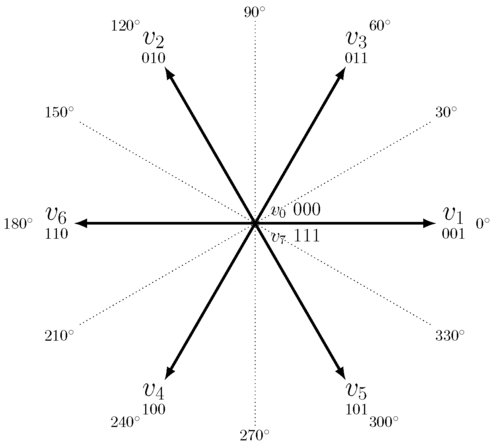
\includegraphics[width=0.75\linewidth]{Basic-Vectors.png}
	\caption{Space vectors \cite{SVPWM_animations}}
	\label{fig:SpaceVectors}
\end{figure}

With the MOSFETs only the bold lined vectors can be created. That is from the center to $+V_{DC}$ and in the other direction (180\degree rotated) $-V_{DC}$. The space between two bold vectors is called a sector. So there are six sectors. To create a vector inbetween the bold vectors the vectors which are the border of a sector should alternate quickly. In each period there is also some time that all phases are either connected to $+V_{DC}$ or $-V_{DC}$ ($v_0$ and $v_7$). By changing the amount of time these $null$ vector are active the magnitude of the generated vector can be controlled. The process of generating a vector in a sector is called Space Vector Modulation (SVM).

\autoref{fig:SvmInSector5} illustrates how a vector in sector 5 is generated. Yngve Solbakken does a great job explaining this image by using animations in his article \cite{SVPWM_animations}.

\begin{figure}[H]
	\centering
	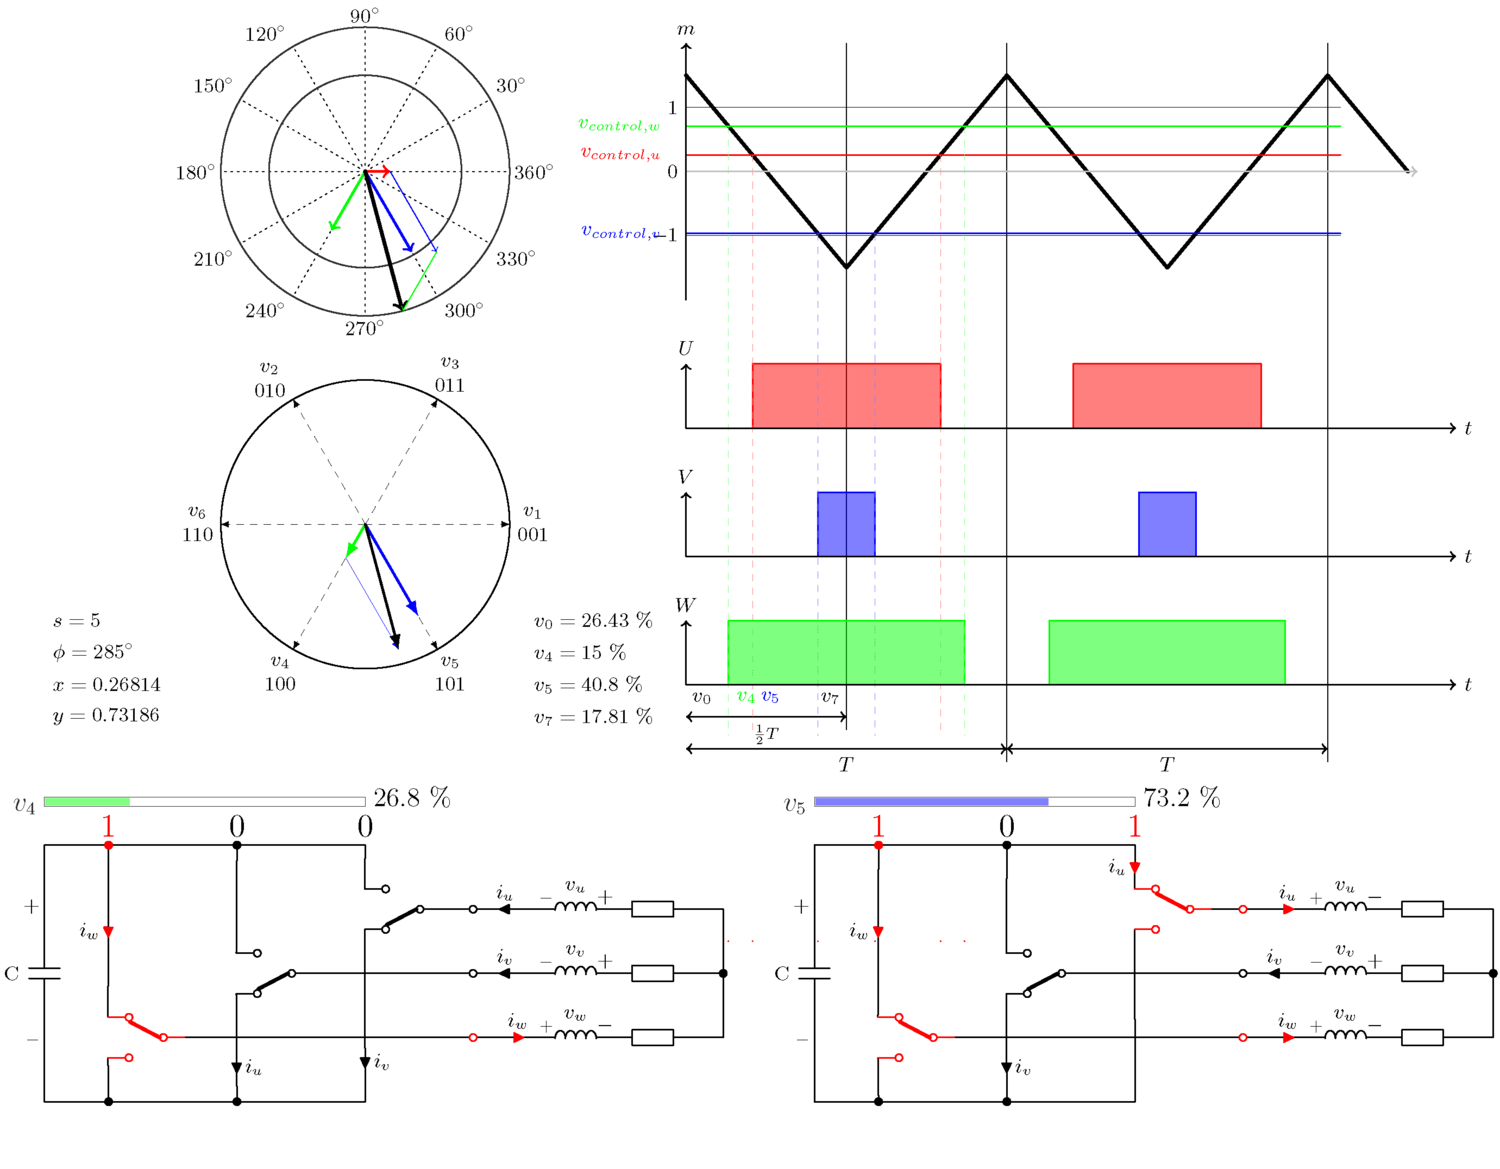
\includegraphics[width=\linewidth]{SVPWM-5.png}
	\caption{SVM in sector 5 \cite{SVPWM_animations}}
	\label{fig:SvmInSector5}
\end{figure}

To calculate the values of $T_1$, $T_2$ and $T_0$ \autoref{eq:SVPWM_Timings} \cite{SVPWM_calculations} can be used. But the triangle compare method explained in \cite{SVPWM_animations} is also possible.

\begin{equation} \label{eq:SVPWM_Timings}
	\begin{split}
		&T_1 = T_s*\frac{\sqrt{3}*V_{ref}}{V_{DC}}*sin(\frac{n}{3}\pi - \phi) \\
		&T_2 = T_s*\frac{\sqrt{3}*V_{ref}}{V_{DC}}*sin(\phi - \frac{n-1}{3}\pi) \\
		&T_0 = T_s - T_1 - T_2 \\
		&\text{n: sector 1 to 6} \\
		&T_s: \text{PWM period}		
	\end{split}
\end{equation}
 
% https://www.researchgate.net/publication/317420242_A_new_space_vector_modulation_strategy_for_three-switch_three-phase_delta_inverter

\chapter{Evaluation criteria}
% How will you be able to determine if your project is successful? Try to find objective and quantitative metrics.

This project will be implemented in Matlab Simulink. FOC controls the speed of a motor.

\section{Response time}
Most FPV drones use motors with a stator diameter of 22mm-24mm and a height of 4mm-8mm and a KV of 2200KV-2800KV. The batteries usually have a voltage between 14,5V (drained 4-cell LiPo) and 25V (full 6-cell LiPo). These FPV drones are used to do quick acrobatic maneuvers which require a quick response of the motor.

The response requirement also depends on size propeller used, the motor size, the 'feel' someone wants their drone to have, etc.

\chapter{Setup}
% What are the signals (real, simulated or physical) that you will use for your project? Whatis the hardware and/or software setup that you have used?

\section{Input}
Normally the Flight Controller (FC) sends (digital) a throttle command to the ESC. This throttle command basically controls the percentage of the duty cycle (and thus voltage applied to the motor) and has a resolution of 2000 steps \cite{DShot_Overview}. By knowing some physical parameters of the motor the RPM can be requested instead.

The input to the complete system is a certain RPM reference. The difference between the requested speed and current speed is converted to a required current using a PID controller. This requested current is then converted to a certain voltage by another PID controller. Eventually the input to the physical system will be a 3-phase voltage.

\section{Feedback}
The feedback signals are the current readings of the motor. These are the currents in the accessible wires which, depending on the motor winding termination, may or may not be equal to the current in the motor phases.

\chapter{Approach}
% A detailed, technical description how you solved the problem.

\section{Dynamic model of a BLDC motor}

\subsection*{Electrical dynamics}
BLDC motors used in FPV drones are almost always delta terminated.

\autoref{fig:DeltaAndStarWoundCircuit} shows the difference between the two windings. At the top there is a 3-phase inverter. Each switch represents a MOSFET which can be controlled by a microprocessor.

\begin{figure}[H]
	\centering
	\begin{subfigure}{0.49\textwidth}
		\centering
		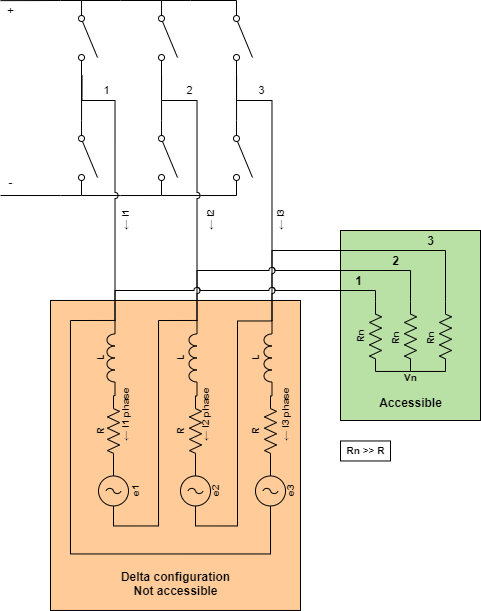
\includegraphics[width=\textwidth]{Draw_IO/BLDC_Dynamics_deltaCircuit.png}
		\caption{Circuit of a 3 phase delta wound BLDC motor}
		\label{fig:DeltaPhaseCircuit}
	\end{subfigure}
	\hfill
	\begin{subfigure}{0.49\textwidth}
		\centering
		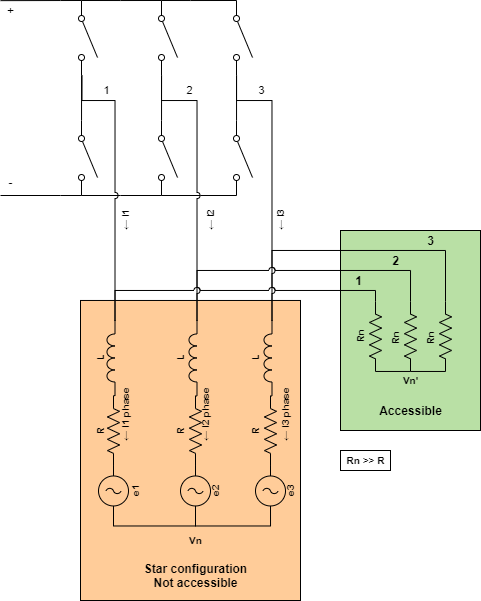
\includegraphics[width=\textwidth]{Draw_IO/BLDC_Dynamics_starCircuit.png}
		\caption{Circuit of a 3 phase star wound BLDC motor}
		\label{fig:StarPhaseCircuit}
	\end{subfigure}
	\caption{Comparison of a delta and star wound BLDC circuit}
	\label{fig:DeltaAndStarWoundCircuit}
\end{figure}

The line-to-line voltage (12, 23, 31) in a delta wound motor is the same as the phase voltage. The equations are shown in \autoref{eq:PhaseVoltageEquationDelta} \cite{BLDC_winding_models}.

\begin{equation} \label{eq:PhaseVoltageEquationDelta}
	\begin{split}
		V_{12} &= RI_{1p} + L\frac{\partial I_{1p}}{\partial t} + M\frac{\partial I_{2p}}{\partial t} + M\frac{\partial I_{3p}}{\partial t} + \omega_m K_e f\left(\theta_e\right) \\
		V_{23} &= RI_{2p} + L\frac{\partial I_{2p}}{\partial t} + M\frac{\partial I_{1p}}{\partial t} + M\frac{\partial I_{3p}}{\partial t} + \omega_m K_e f\left(\theta_e - \frac{2pi}{3}\right) \\
		V_{31} &= RI_{3p} + L\frac{\partial I_{3p}}{\partial t} + M\frac{\partial I_{1p}}{\partial t} + M\frac{\partial I_{2p}}{\partial t} + \omega_m K_e f\left(\theta_e - \frac{4pi}{3}\right)
	\end{split}
\end{equation}

The equations for the star configuration are similar (\autoref{eq:PhaseVoltageEquationStar}). The main difference is that the phase voltage is the difference between the neutral and 'input' voltage

\begin{equation} \label{eq:PhaseVoltageEquationStar}
	\begin{split}
		V_{1n} &= RI_{1} + L\frac{\partial I_{1}}{\partial t} + M\frac{\partial I_{2}}{\partial t} + M\frac{\partial I_{3}}{\partial t} + \omega_m K_e f\left(\theta_e\right) \\
		V_{2n} &= RI_{2} + L\frac{\partial I_{2}}{\partial t} + M\frac{\partial I_{1}}{\partial t} + M\frac{\partial I_{3}}{\partial t} + \omega_m K_e f\left(\theta_e - \frac{2pi}{3}\right) \\
		V_{3n} &= RI_{3} + L\frac{\partial I_{3}}{\partial t} + M\frac{\partial I_{1}}{\partial t} + M\frac{\partial I_{2}}{\partial t} + \omega_m K_e f\left(\theta_e - \frac{4pi}{3}\right)
	\end{split}
\end{equation}

Where the neutral voltage is given in \autoref{eq:NeutralVoltageEquation}

\begin{equation} \label{eq:NeutralVoltageEquation}
	\begin{split}
		V_{n0} &= \frac{\left(V_{10} + V_{20} + V_{30} \right) - \left(\omega_m K_e f\left(\theta_e\right) + \omega_m K_e f\left(\theta_e - \frac{2pi}{3}\right) + \omega_m K_e f\left(\theta_e - \frac{4pi}{3}\right) \right)}{3}
	\end{split}
\end{equation}

\begin{equation*}
	\begin{split}
		I_{1p, 2p, 3p} &= \text{phase currents} \\
		I_{1, 2, 3} &= \text{line currents} \\
		V_{10, 20, 30, n0} &= \text{voltage refenced to ground} \\
		R &= \text{phase resistance} \\
		L &= \text{phase inductance} \\
		M &= \text{mutural inductance between phases} \\
		K_e &= \text{Back EMF constant} \\
		f() &= \text{Back EMF function (trapezoidal or sinusoidal). Can also be written as: } f_i\left(\theta_e - (i - 1)*\frac{2\pi}{3}\right) \\
		\omega_m &= \text{mechanical angular speed} \\
		\theta_e &= \text{electrical rotor angle}
	\end{split}
\end{equation*}

The BEMF in a phase $i$ can also be written as \autoref{eq:BackEMFShorthand}. 

\begin{equation} \label{eq:BackEMFShorthand}
	e_i = \omega_m K_e f_i\left(\theta_e - (i - 1)*\frac{2\pi}{3}\right)
\end{equation}

The input currents in the delta configuration can be described as in \autoref{eq:DeltaInputCurrents} (considering the direction of thee current as shown in \autoref{fig:DeltaAndStarWoundCircuit}).

\begin{equation} \label{eq:DeltaInputCurrents}
	\begin{split}
	I_1 = I_{1p} - I_{3p} \\
	I_2 = I_{2p} - I_{1p} \\
	I_3 = I_{3p} - I_{2p}
	\end{split}
\end{equation}

The input current in a star configuration is the same as the phase current. So in a star terminated motor the phase currents can be directly measured. In a delta connected motor not.

\subsection*{Physical dynamics}
The physical dynamics are shown in \autoref{eq:ElectricalTorqueEquations} \cite{BLDC_winding_models}.

\begin{equation} \label{eq:ElectricalTorqueEquations}
	\begin{split}
		T_e &= J\frac{\partial \omega_m}{\partial t} + B\omega_m + T_l \\
		T_e &= \sum_{i=1}^{3}\left(I_{ip}K_tf_i\left(\theta_e - (i - 1)*\frac{2\pi}{3}\right)\right) \\
		\frac{\partial \theta_e}{\partial t} &= \omega_e = p\omega_m
	\end{split}
\end{equation}

\begin{equation*}
	\begin{split}
		J &= \text{moment of inertia} \\
		B &= \text{friction coefficient} \\
		T_l &= \text{load torque} \\
		T_e &= \text{electrical torque} \\
		K_t &= \text{torque constant} \\
		f() &= \text{Back EMF function (trapezoidal or sinusoidal)} \\
		\omega_m &= \text{mechanical angular speed} \\
		\omega_e &= \text{electrical angular speed} \\
		\theta_e &= \text{electrical rotor angle} \\
		p &= \text{number of pole pairs in the rotor}
	\end{split}
\end{equation*}

\subsection*{State space for a delta wound motor}
The states of the system are all the dynamical components of the system and are given in \autoref{eq:SystemStates}.

\begin{equation}\label{eq:SystemStates}
	x = \begin{bmatrix} I_{1p} \\ I_{2p} \\ I_{3p} \\ \omega_m \\ \theta_e \end{bmatrix}
\end{equation}

The inputs are the line voltages and the load torque (\autoref{eq:SystemInputs}). The line voltages can be controlled using PWM on the MOSFETS. The load torque is for example the resistance of a rotating propeller.

\begin{equation}\label{eq:SystemInputs}
	u = \begin{bmatrix} V_{1} \\ V_{2} \\ V_{3} \\ T_l \end{bmatrix}
\end{equation}

The output are stated in \autoref{eq:SystemOutputs}. Only the currents and voltages going in and out to the motor can be measured in a sensorless BLDC system. Since the voltage is the input this is already known.

\begin{equation}\label{eq:SystemOutputs}
	y = \begin{bmatrix} I_{1} \\ I_{2} \\ I_{3} \end{bmatrix}
\end{equation}

Writing the system dynamics in term of $\dot{x} = Ax + bu$ gives the matrices shown in \autoref{eq:SystemMatricesDelta}. For simplicity the mutual inductance (M) is set to 0.

\begin{equation}\label{eq:SystemMatricesDelta}
	\begin{split}
	A &= \begin{bmatrix}
			-\frac{R}{L} && 0 && 0 && -\frac{K_e f\left(\theta_e\right)}{L} && 0 \\
			0 && -\frac{R}{L} && 0 && -\frac{K_e f\left(\theta_e - \frac{2pi}{3}\right)}{L} && 0 \\
			0 && 0 && -\frac{R}{L} && -\frac{K_e f\left(\theta_e - \frac{4pi}{3}\right)}{L} && 0 \\
			\frac{K_t f\left(\theta_e\right)}{J} && \frac{K_t f\left(\theta_e - \frac{2pi}{3}\right)}{J} && \frac{K_t f\left(\theta_e - \frac{4pi}{3}\right)}{J} && - \frac{B}{L} && 0 \\
			0 && 0 && 0 && p && 0
		 \end{bmatrix} \\
	 B &= \begin{bmatrix}
	 		\frac{1}{L} && -\frac{1}{L} && 0 && 0 \\
	 		0 && \frac{1}{L} && -\frac{1}{L} && 0 \\
	 		-\frac{1}{L} && 0 && \frac{1}{L} && 0 \\
	 		0 && 0 && 0 && -\frac{1}{J} \\
	 		0 && 0 && 0 && 0
	 	\end{bmatrix} \\
 	C &= \begin{bmatrix}
	 		1 && 0 && -1 && 0 && 0 \\
	 		-1 && 1 && 0 && 0 && 0 \\
	 		0 && -1 && 1 && 0 && 0
 		\end{bmatrix}
 	\end{split}
\end{equation}

The dynamics are thus as shown in \autoref{eq:SystemDynamics}.

\begin{equation}\label{eq:SystemDynamics}
	\begin{split}
	\dot{I}_{1p} &= \frac{1}{L} \left( -I_{1p} R - \omega_m K_e f\left(\theta_e\right) + V_1 - V_2 \right) \\
	\dot{I}_{2p} &= \frac{1}{L} \left( -I_{2p} R - \omega_m K_e f\left(\theta_e - \frac{2pi}{3}\right) + V_2 - V_3 \right) \\
	\dot{I}_{3p} &= \frac{1}{L} \left( -I_{3p} R - \omega_m K_e f\left(\theta_e - \frac{4pi}{3}\right) + V_3 - V_1 \right) \\
	\dot{\omega}_m &= \frac{K_t}{J} \left( I_{1p} f\left(\theta_e\right) + I_{2p} f\left(\theta_e - \frac{2pi}{3}\right) + I_{3p} f\left(\theta_e - \frac{4pi}{3}\right) \right) - \omega_m \frac{B}{L} \\
	\dot{\theta}_e &= p \omega_m
 	\end{split}
\end{equation}

Note that the BEMF function ($f()$) has a varying output value based on the current electrical rotor angle ($\theta_e$). The function has either a trapezoidal or sinusoidal waveform, depending on the motor windings. This system is thus nonlinear. BLDC motors are generally considered to have a trapezoidal BEMF waveform. However, when measuring the BEMF of a BLDC motor used in an FPV drone rotated by hand with a virtual neutral point as the reference the BEMF looked more sinusoidal as seen in \autoref{fig:BemfVirtualNeutralHandSpinning}.

\begin{figure}[H]
	\centering
	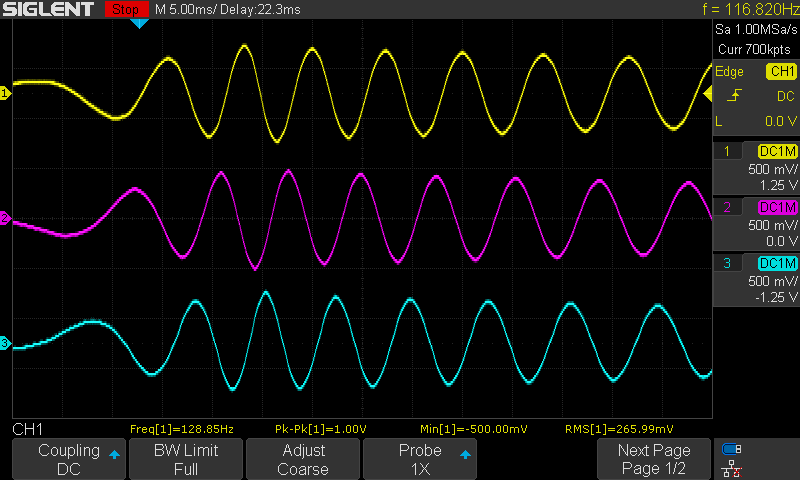
\includegraphics[width=\textwidth]{Scope/VirtualNeutral/BEMF_Phases_virtual_neutral.png}
	\caption{Measurement of the Back EMF over the resistor in series with a phase/line with the virtual neurtal point as the reference of a Emax Eco 2306 1700kv motor when spinning the motor by hand.}
	\label{fig:BemfVirtualNeutralHandSpinning}
\end{figure}

The only equilibrium point (all derivatives of the states are zero while the input is also zero) in this state space model is when all states are 0. Meaning that the motor is at standstill. Linearizing about this equilibrium point is thus not very useful since only at startup the motor is at standstill and a linearized model is only valid within a certain margin of the equilibrium point.During operation the derivatives of the phase currents are constantly changing.

\section{Model in Simulink}

The equations shown in \autoref{eq:SystemMatricesDelta} can be implemented in Simulink as shown in \autoref{fig:SimulinkNonlinearModel}. The Matlab function called "SystemDynamics" Implements the multiplication of the A and state matrices. 

\begin{figure}[H]
	\centering
	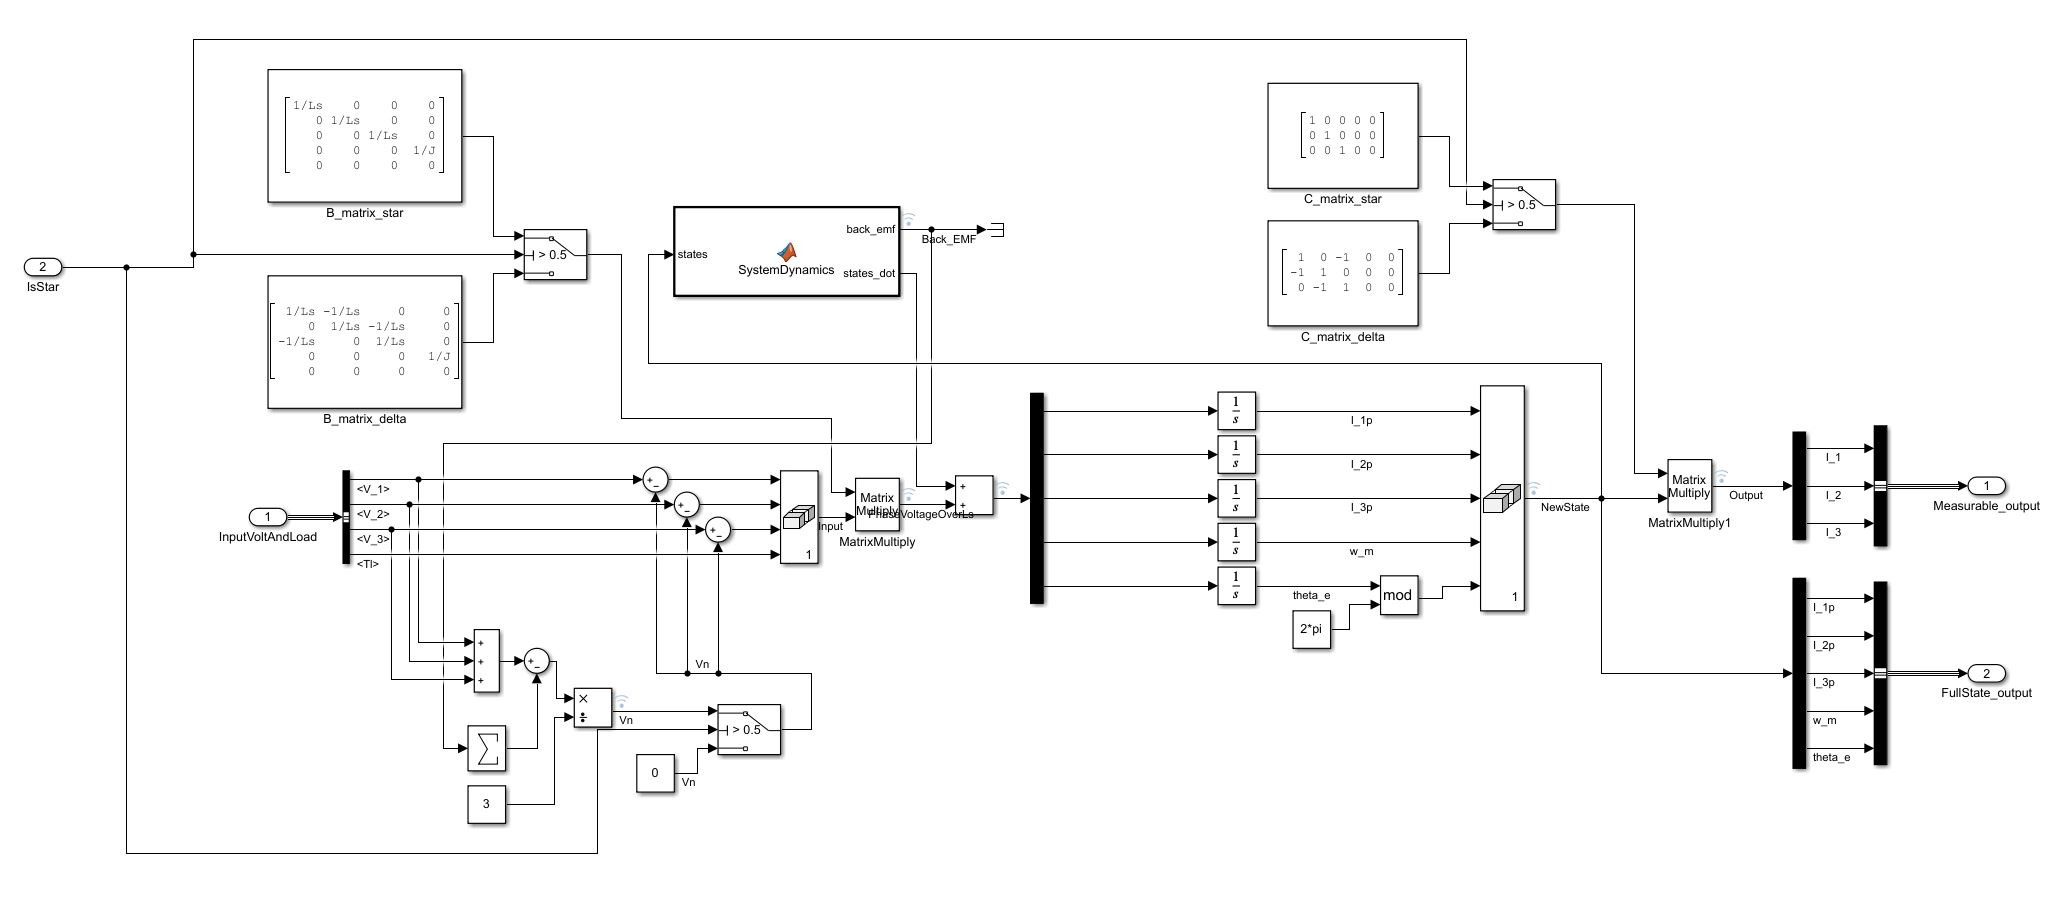
\includegraphics[width=\textwidth]{Matlab/SimulinkNonlinearModel_StarAndDelta.JPG}
	\caption{The continuous implementation of BLDC motor}
	\label{fig:SimulinkNonlinearModel}
\end{figure}

To see if the system behaves as expected a short load torque pulse is given to the system while the input voltage on phase 1, 2 and 3 are all 0V (and the Delta termination is used). The expectation is that the angular velocity ($\omega_m$) will rise quickly and then reduce to 0 over time. Also the Back EMF and current is expected to rise quickly and then reduce to 0 again over time. The system is implement to generate both sinusoidal and trapezoidal Back EMF waveforms. The system behaves as expected as shown in \autoref{fig:TorqueInputResponse}. It can be seen that with a trapezoidal Back EMF waveform the system slows down quicker.

\begin{figure} [H]
	\centering
	\begin{subfigure}{0.80\textwidth}
		\centering
		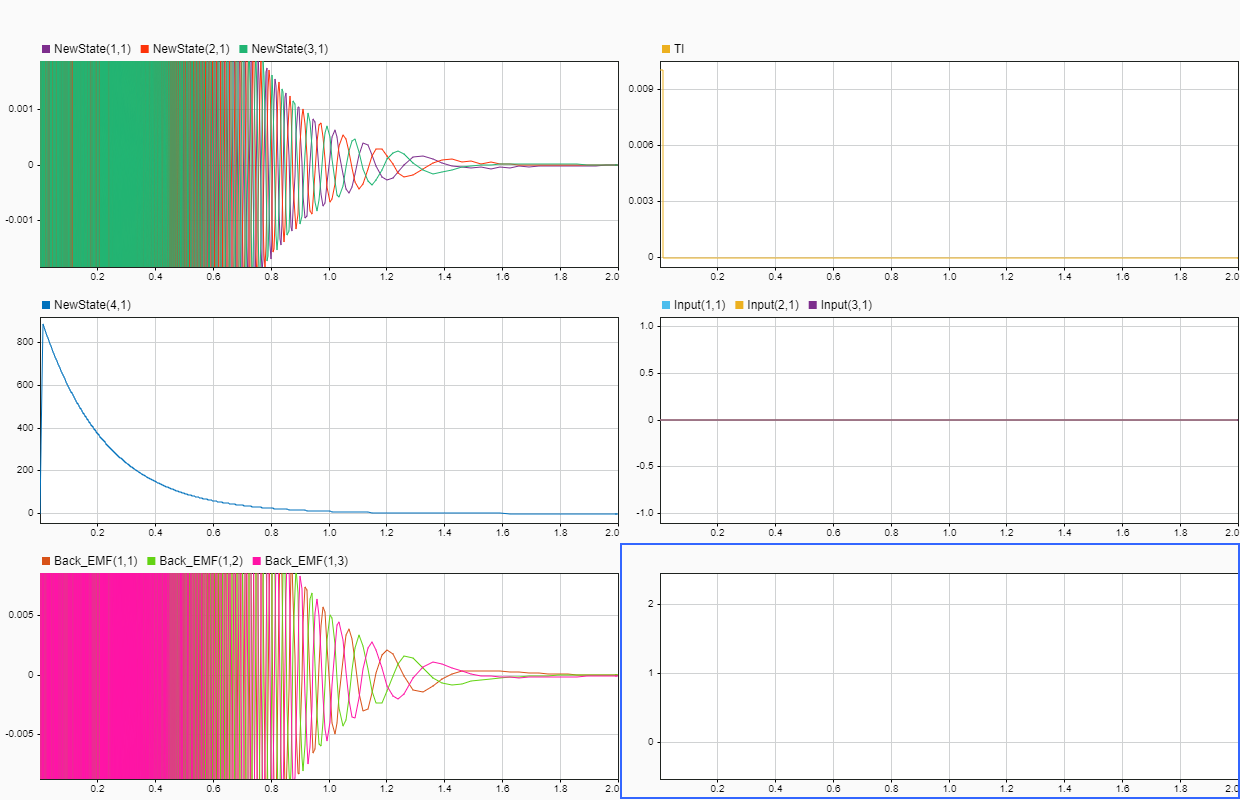
\includegraphics[width=\textwidth]{Matlab/TorqueInputPulse_SinusoidalBackEMF.png}
		\caption{Torque input pulse response with sinusoidal Back EMF}
		\label{fig:TorqueInputResponseSinusoidal}
	\end{subfigure}
	\hfill
	\begin{subfigure}{0.80\textwidth}
		\centering
		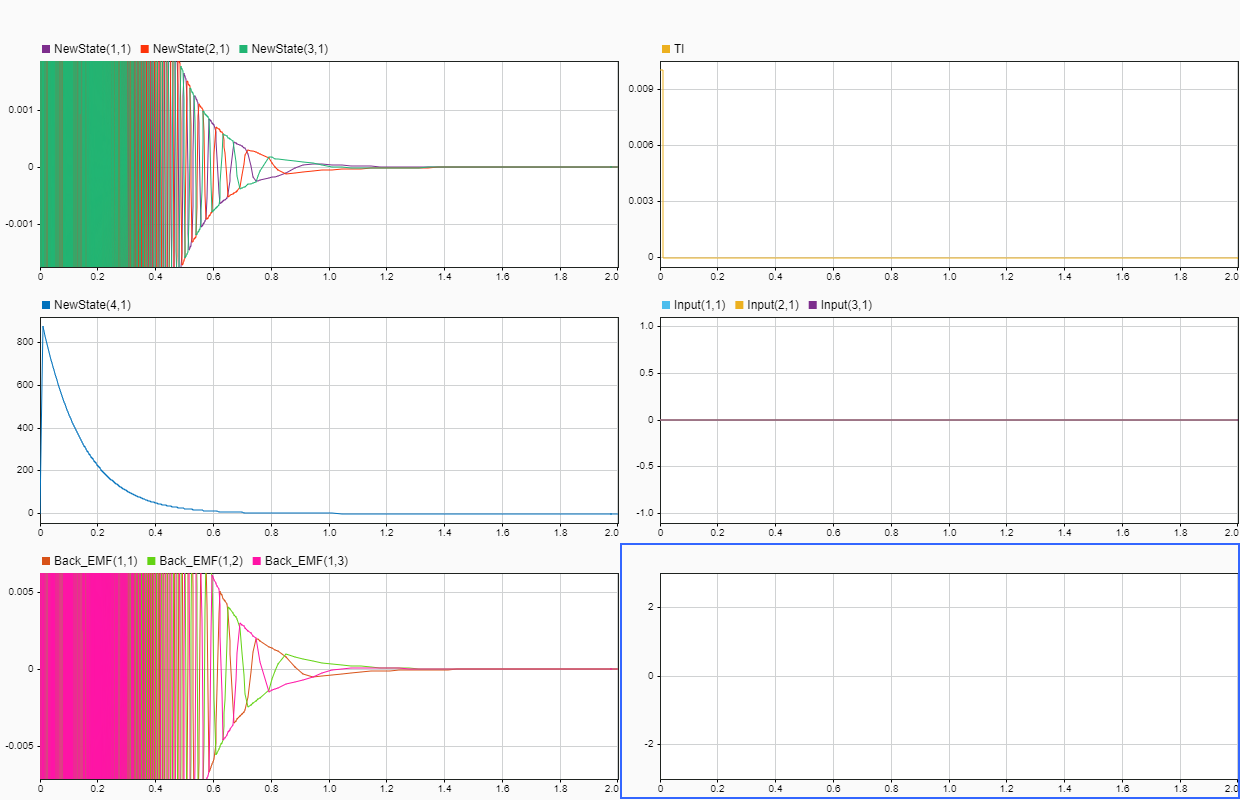
\includegraphics[width=\textwidth]{Matlab/TorqueInputPulse_TrapezoidalBackEMF.png}
		\caption{Torque input pulse response with trapezoidal Back EMF}
		\label{fig:TorqueInputResponseTrapezoidal}
	\end{subfigure}
	\caption{Torque input pulse response with sinusoidal and trapezoidal Back EMF. For both figures: left-top) phase currents, left-middle) angular velocity, left-bottom) Back EMF, right-top) torque input, right-middle) input voltages.}
	\label{fig:TorqueInputResponse}
\end{figure}

\section{Dynamic model of a BLDC motor in the DQ-frame}
when a 3-phase motor is rotating the phase currents and voltages are constantly changing in a sinusoidal fashion. Using the Clarke and Park transformations these sinusoids can be mapped into the DQ frame in which the values are constant. For the park transformation the electrical rotor angle ($\theta_e$) is needed.

When the measured phase currents are transformed to the DQ-frame, PI controllers can be used. One for the D-axis, one for the Q-axis and one for the speed (see \autoref{fig:SimulinkDqControl}).

\begin{figure}[H]
	\centering
	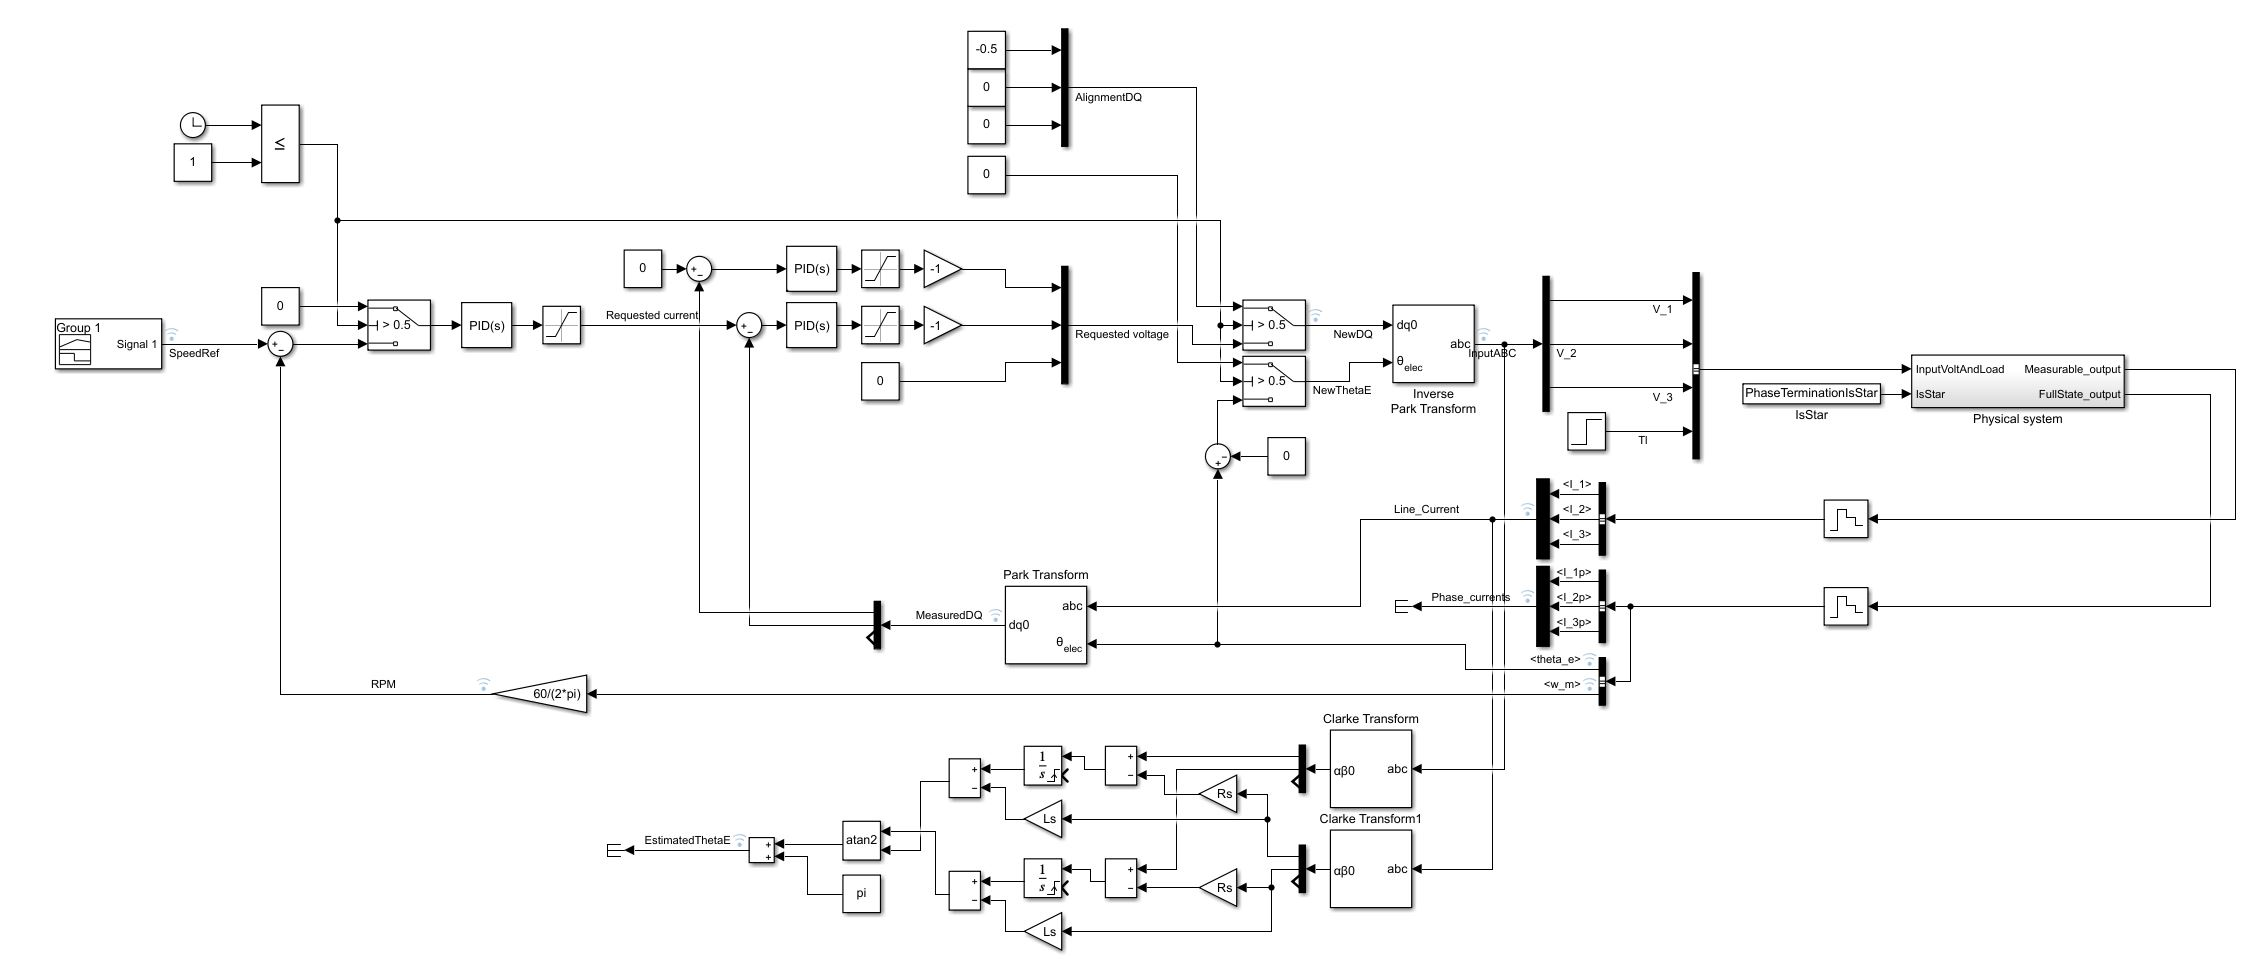
\includegraphics[width=\textwidth]{Matlab/SimulinkNonlinearModelDQ_Control.JPG}
	\caption{DQ control of the BLDC motor model.}
	\label{fig:SimulinkDqControl}
\end{figure}

This model omits the SVM part since it effectively will produce the same voltages over the phases.

After tuning the PI controllers, a reference speed can be followed as seen in \autoref{fig:DQ_SpeedRefStarMotor}. The simulated Maxon motor \cite{Maxon_motor_EC_14} has a Kv of 1890 (rpm/V). In the graphs is can be seen that at an RPM of around 1890 the applied voltage is indeed around 1V.

\begin{figure}[H]
	\centering
	\begin{subfigure}{\textwidth}
		\centering
		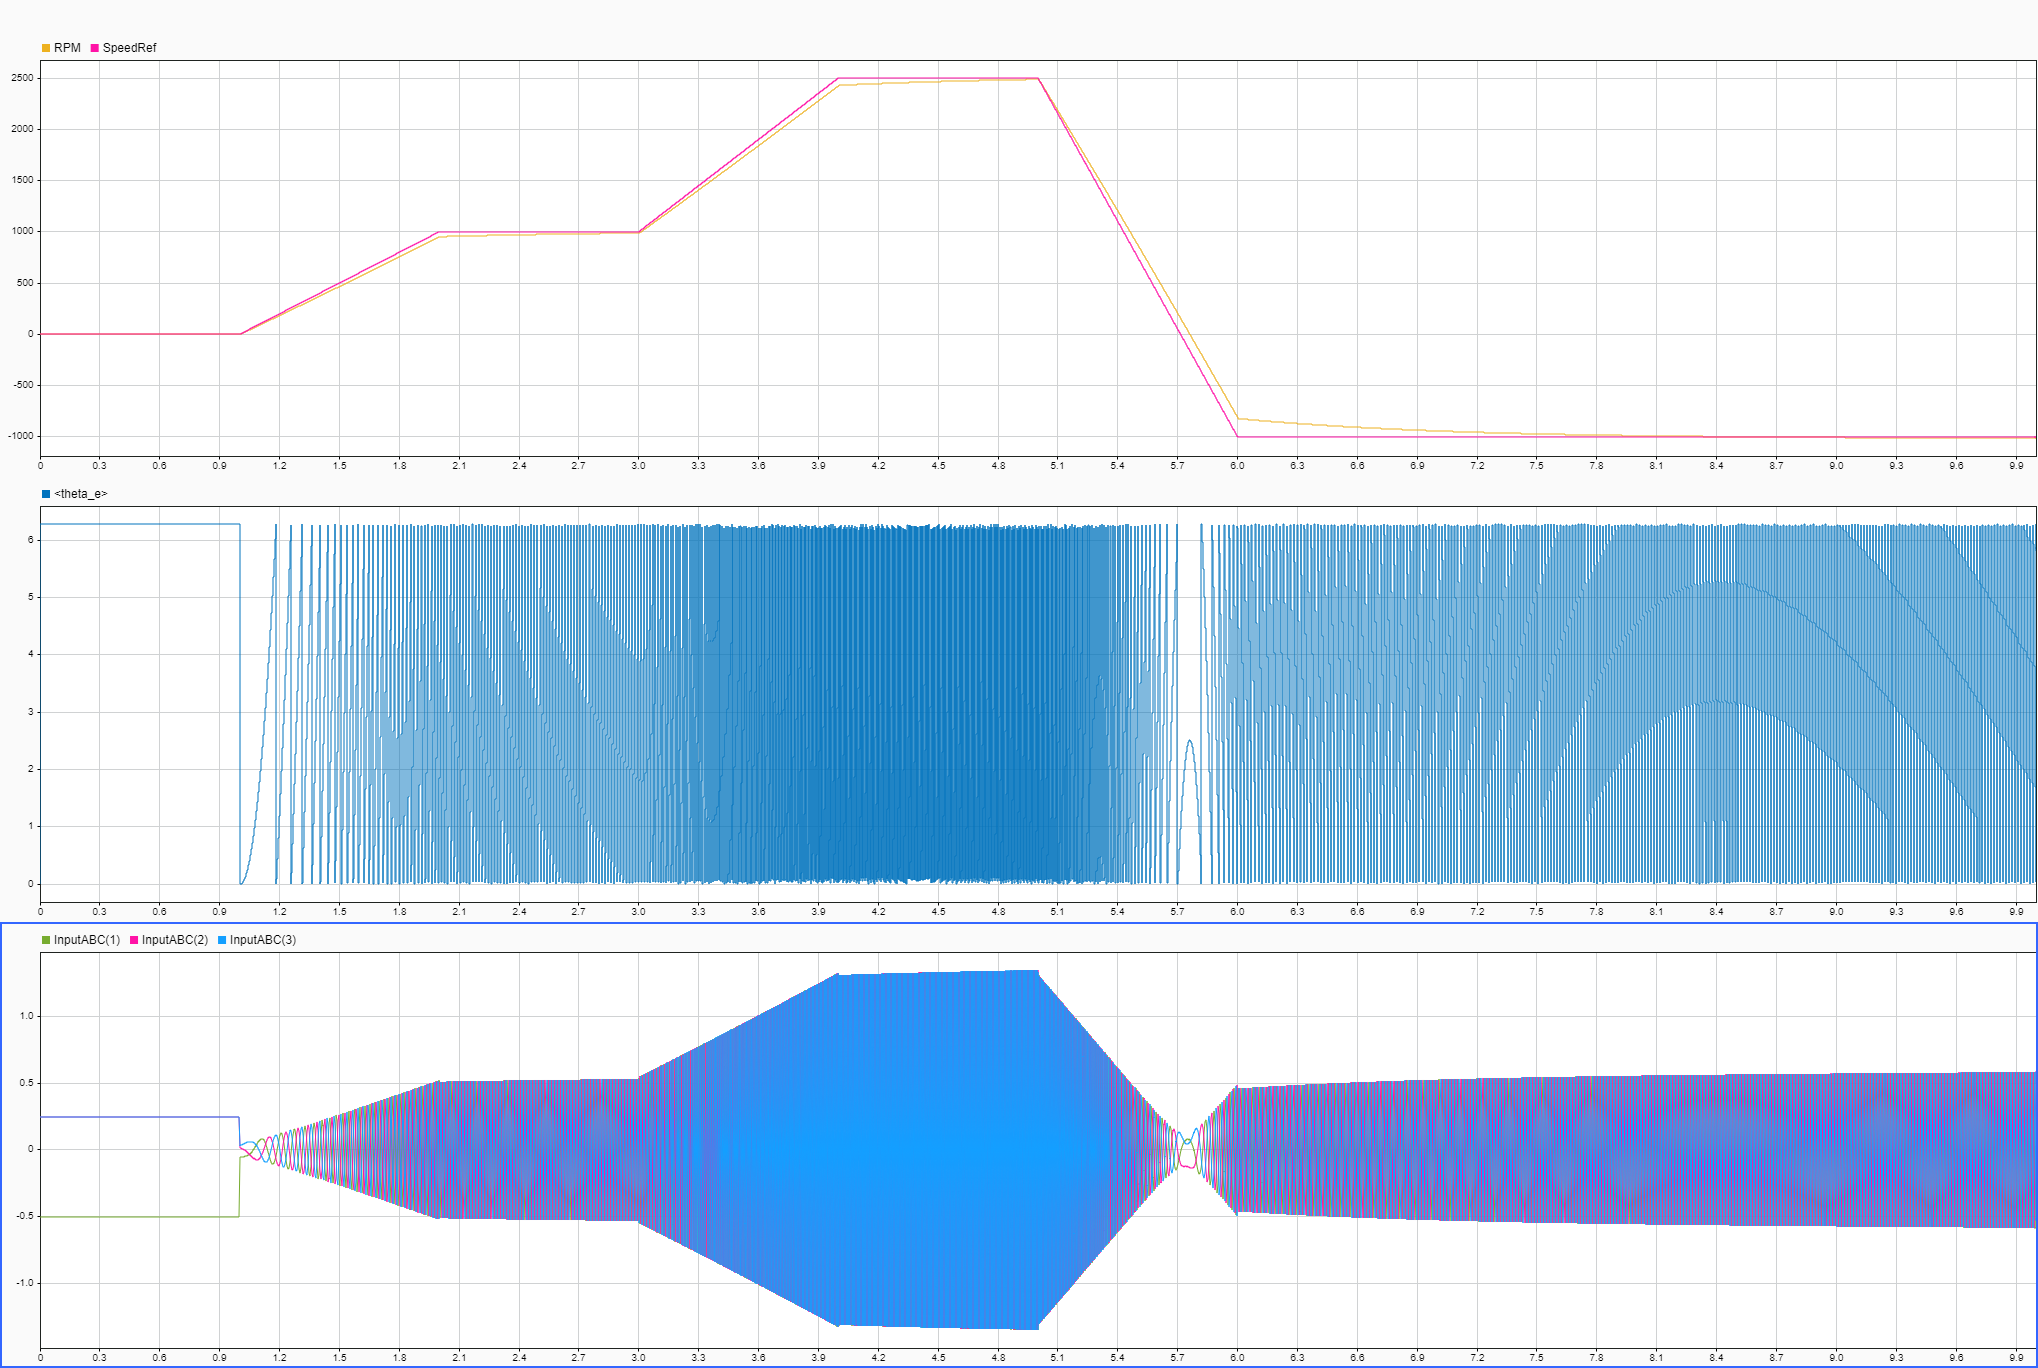
\includegraphics[width=\textwidth]{Matlab/SpeedRefFollowStar.png}
		\caption{}
		\label{fig:SpeedRefFollowMaxon}
	\end{subfigure}
	\hfill
	\begin{subfigure}{\textwidth}
		\centering
		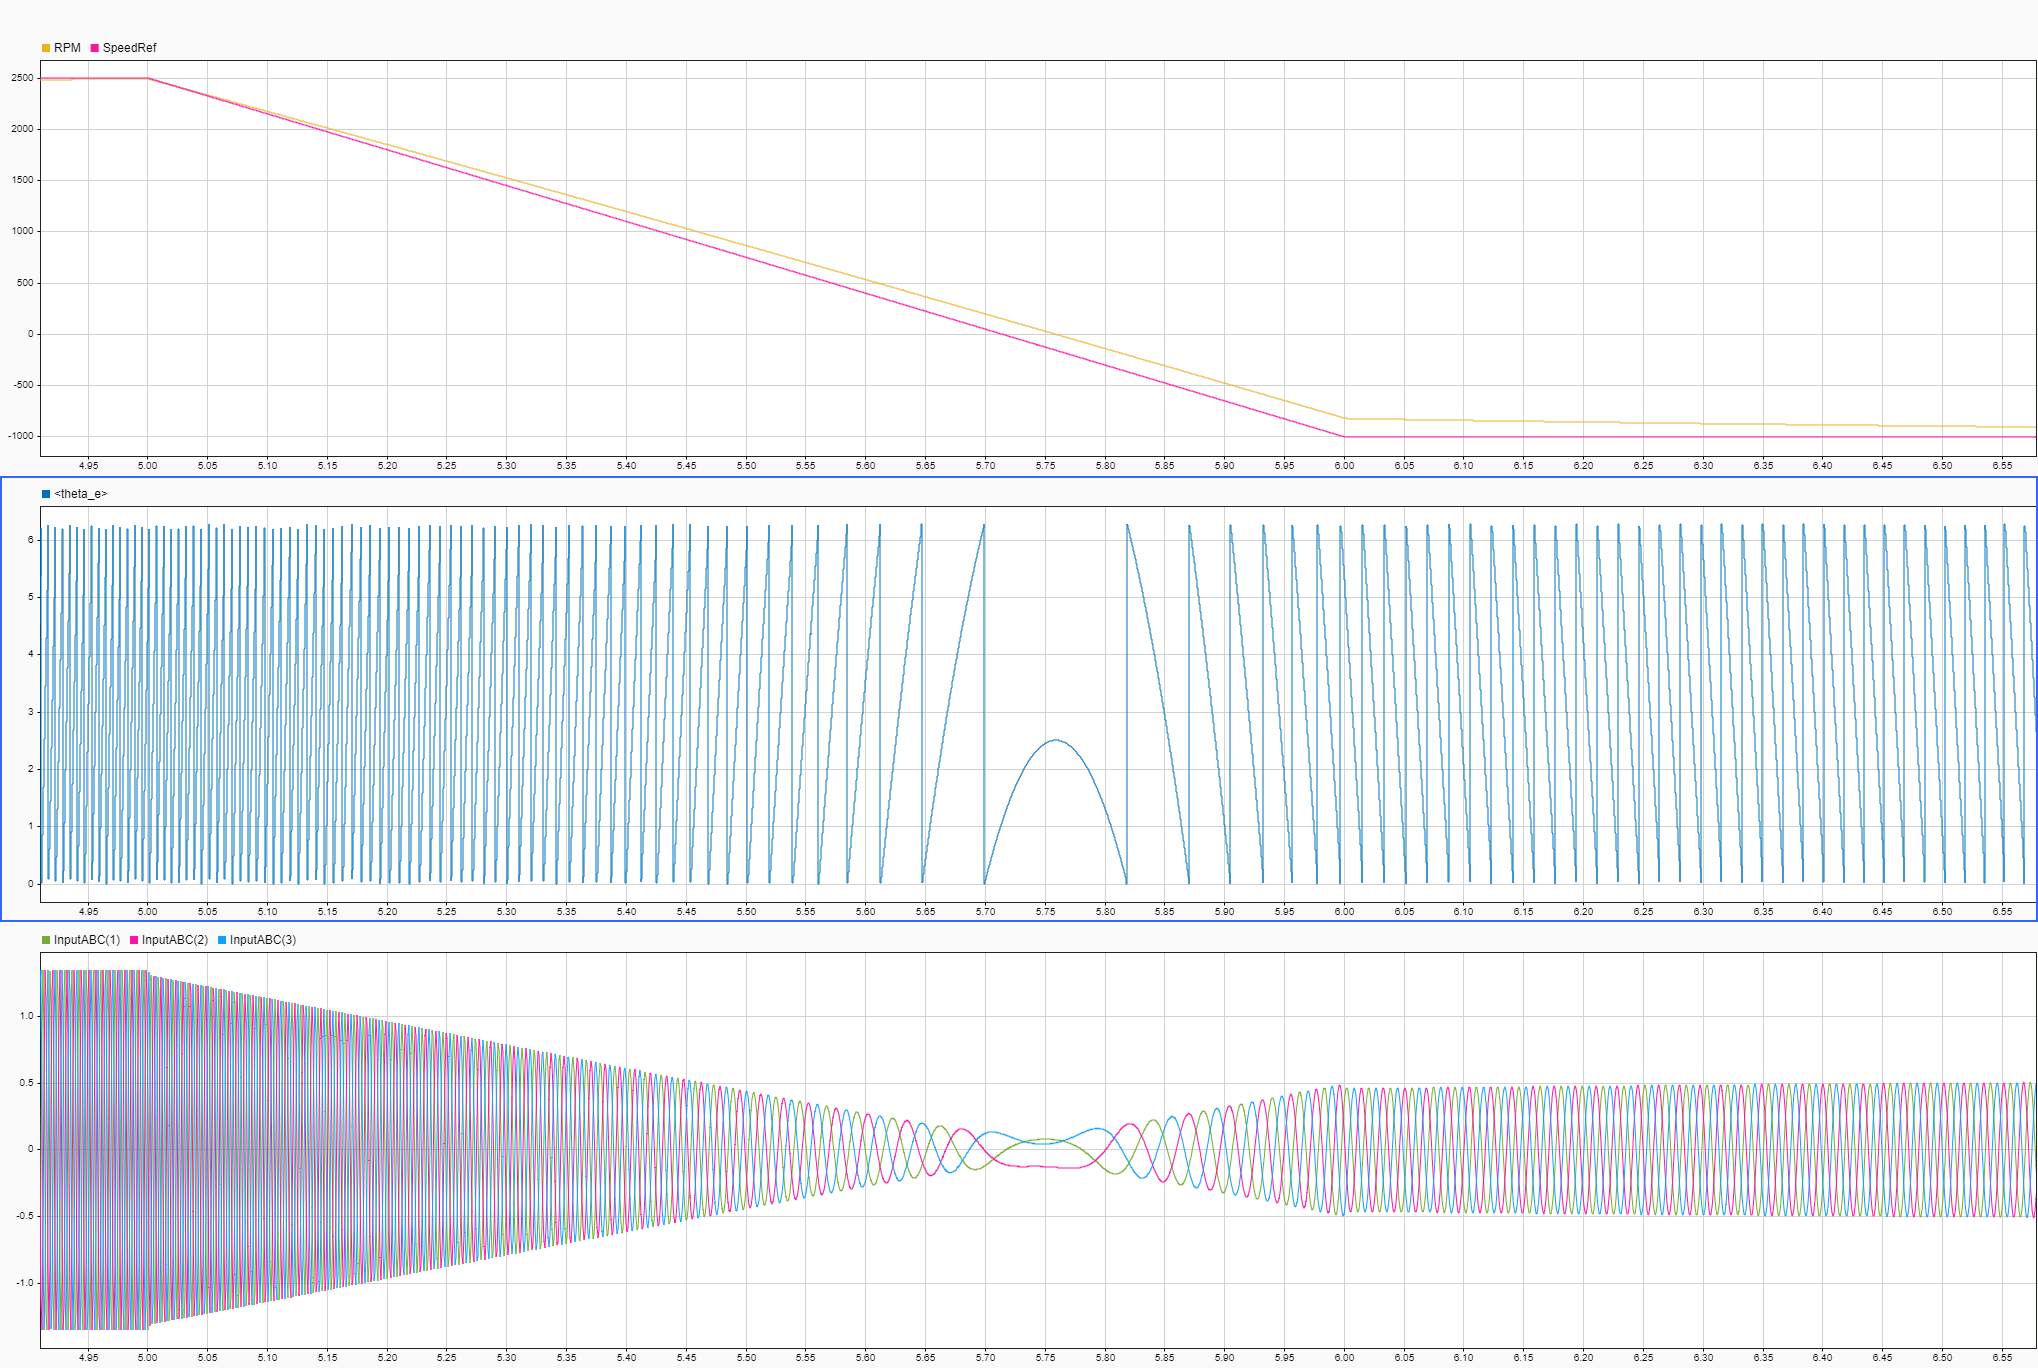
\includegraphics[width=\textwidth]{Matlab/SpeedRefFollowStar_ZoomedDirectionChange.png}
		\caption{Zoomed in on the direction change moment}
		\label{fig:SpeedRefFollowMaxonDirectionChangeZoom}
	\end{subfigure}
	\caption{Simulating the Maxon EC 14 flat 12V (339252) BLDC motor \cite{Maxon_motor_EC_14} with a star termination to follow a certain speed reference. In both images the top graph shows the reference speed and measured speed. The middle graph shown the electrical angle. The bottom graph shown the input voltages.}
	\label{fig:DQ_SpeedRefStarMotor}
\end{figure}

For this reference speed tracker the angle and speed of the state space model are used. When calculating the angle using the integration method described in \autoref{seq:RotorPositionEstimationIntegration} the angle looks like the actual angle, but is not correct as can be seen in \autoref{fig:EstimatedRotorPositionWithIntegration}.

\begin{figure}[H]
	\centering
	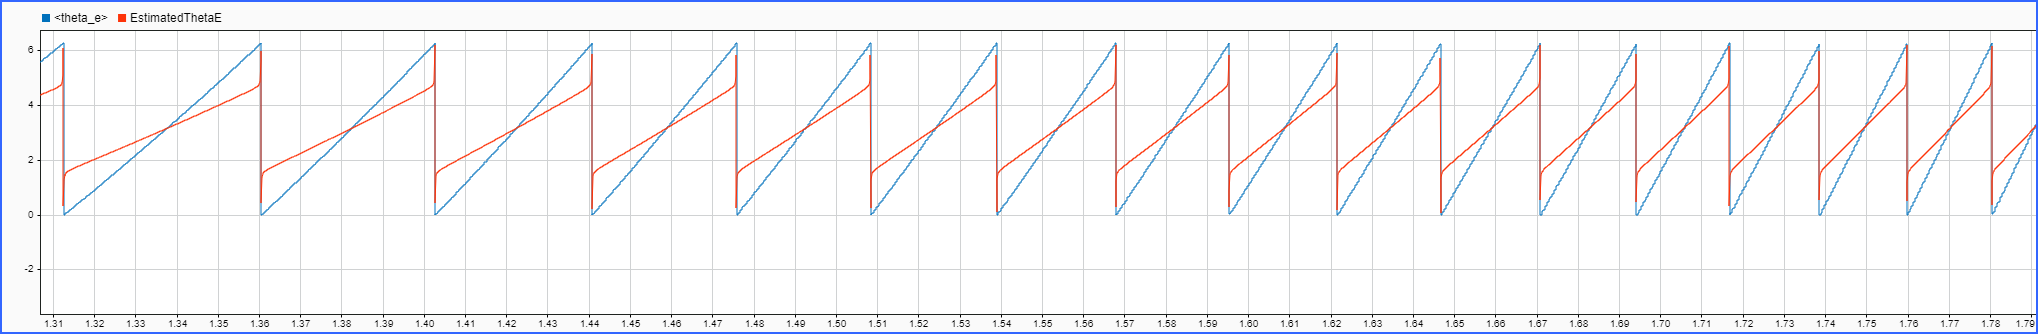
\includegraphics[width=\textwidth]{Matlab/Estimated_ThetaE_FluxIntegration.png}
	\caption{Estimated rotor angle vs actual rotor angle}
	\label{fig:EstimatedRotorPositionWithIntegration}
\end{figure}
	
\chapter{Results and analysis}
% Evaluation of the results using the defined criteria and a reflection on theoutcomes, explanations for shortcomings, ideas for improvements.

In this project a dynamical motor model has been implemented in Matlab of which the speed can be controlled by making use of the Clarke and Park transformations.

This speed reference tracking did make use of the speed and rotor angle outputs of the state space. Normally in a sensorless algorithm these values are of course not available. However, it does show that, if sensors are used, the speed can be controlled with PID controllers and the Clarke and Park transformations.

It turned out that the rotor angle estimation integration technique did not work as well as was expected. A better method would be to use something like a Sliding Mode Observer (SMO) or an Unscented Kalman Filter (UKF). Both or which are used to estimate/observe nonlinear systems.

\chapter{Conclusions}
% (Short) What did you learn from doing the project? What solutions did you provide?

What I learned from the project is that in order to design a controller, a good understanding is needed of the system to be controlled. During this project I 'waisted' a lot of time learning about different types of motor, how these differences influence the operation of the system and about FOC. If I had more preknowledge about the electrical and physical aspects of the motor and FOC I think that I would have spend my time more efficiently on the actual control aspects.

Once I learned that I had to use something like SMO or UKF there was only so much time left which meant that I couldn't fully learn how to implement these systems in my project in time.

\printbibliography


\end{document}